% !TEX root = ../tex/3-1.tex
% 第3章：本文は青、補足は緑
\newcommand{\asmain}{%
    \setbeamercolor{frametitle}{fg=white,bg=main}%
    \setbeamercolor{structure}{fg=main}%
    \setbeamercolor{itemize item}{fg=main}%
    \setbeamercolor{itemize subitem}{fg=main}%
    \setbeamercolor{enumerate item}{fg=main}%
}
\newcommand{\assuppl}{%
    \setbeamercolor{frametitle}{fg=white,bg=examplecol}%
    \setbeamercolor{structure}{fg=examplecol}%
    \setbeamercolor{itemize item}{fg=examplecol}%
    \setbeamercolor{itemize subitem}{fg=examplecol}%
    \setbeamercolor{enumerate item}{fg=examplecol}%
}
% フレームタイトルの「補足」だけを□で囲む
\newcommand{\supplmark}{%
    \setlength{\fboxsep}{1.5pt}%
    \setlength{\fboxrule}{0.7pt}%
    \fbox{\textbf{補足}}%
}
\asmain


%=============================================

\begin{frame}{第2章から第3章へ}
    \begin{block}{これまでの見方}
        第2章では、VAEの枠組みを使って、データに少しずつノイズを加える過程を固定\\
        その逆のノイズを取り除く過程をどう学習するかを見てきた
    \end{block}
    \begin{block}{ここからの見方}
        同じく基礎的な第二の視点として、
        エネルギーベースモデル（EBM）からスコアへ進む。
    \end{block}
    \begin{itemize}
        \item EBMは、データのある領域でエネルギーが低く、
        ない領域で高くなる関数で分布を表す
        \item サンプリングには、その勾配であるスコアを使う
        \item スコアがわかれば、正規化定数なしで生成できる
    \end{itemize}
    \vfill
    \footnotesize
    Ackley et al.\ (1985), LeCun et al.\ (2006)
\end{frame}
%=============================================
\asmain
\begin{frame}{三つの視点と第3章の位置}
    \centering
    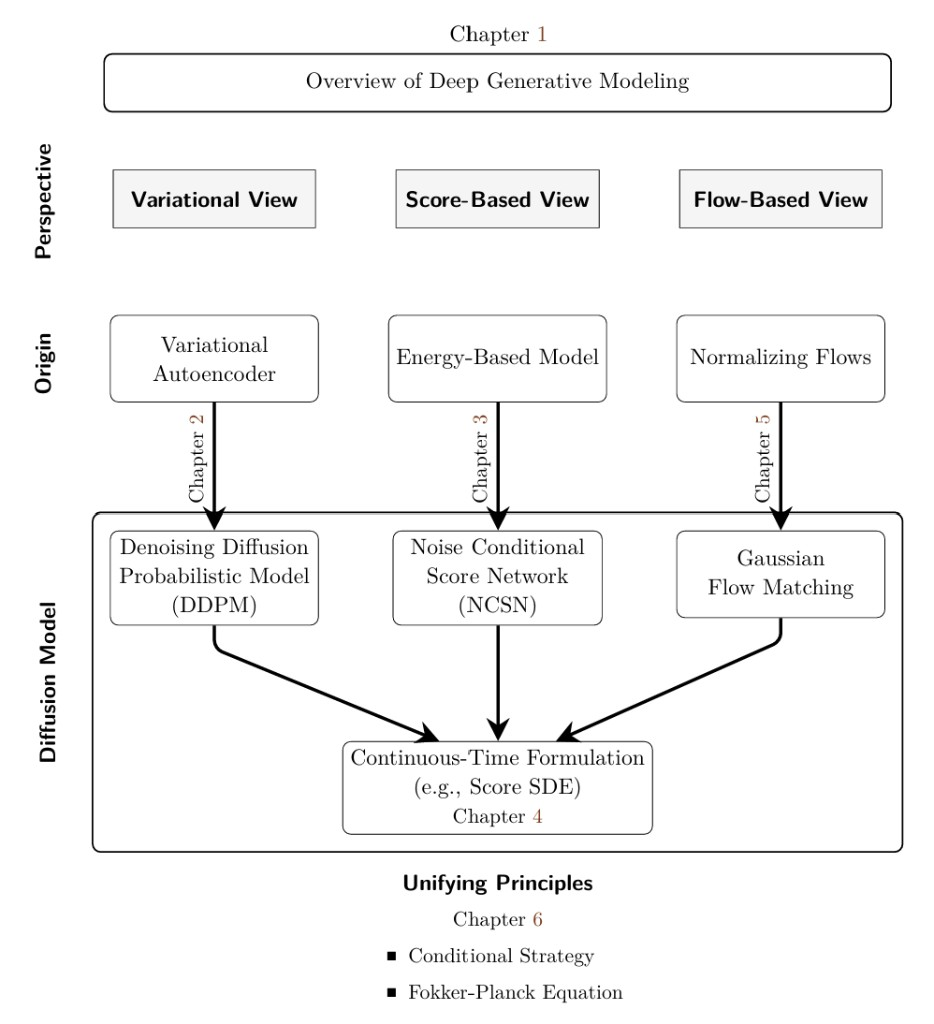
\includegraphics[height=0.78\textheight,keepaspectratio]{perspectives.jpg}
    \vfill
    この章は中央の列である。EBMからNCSNへ進み、第4章の連続時間へつながる。
\end{frame}
%=============================================
\asmain
\begin{frame}{3.1 の位置づけ}
    \begin{block}{この節の役割}
        拡散モデルをスコアの視点から読むための橋渡し
    \end{block}
    \begin{enumerate}
        \item \textbf{3.1.1:スコアベースモデリングの基礎理解}\\ 
        エネルギー関数で分布を表す。
        最尤学習がなぜ難しいかを見る
        \item \textbf{3.1.2:DSM(Diffusion Score Matching)からスコアへ} \\
        スコア関数を定義し、
        密度そのものではなくスコアを学ぶ理由を見る
        \item \textbf{3.1.3:NCSN(Noise Conditional Score Network)}\\
         スコアマッチング
        \item \textbf{3.1.4} ランジュバン動力学
    \end{enumerate}
    \vfill
    今回は3.1.4までを扱う。
\end{frame}
%=============================================
\section{3.1.1 エネルギー関数によるモデル化}
\asmain
\begin{frame}{区切り：3.1.1 エネルギー関数によるモデル化}
    \tableofcontents[currentsection]
\end{frame}
%=============================================
\asmain
\begin{frame}{3.1.1 エネルギー関数で分布を表す}
    エネルギーベースモデル(EBM)は、エネルギー関数で分布を表すモデルである。
    \[
    p_\phi(\bm{x}):=
    \frac{\exp\!\bigl(-E_\phi(\bm{x})\bigr)}{Z_\phi}
\]
    \begin{block}{エネルギー関数}
        $\bm{x}\in\mathbb{R}^{D}$に対し、モデルがどのくらい「ありそう」かを表すスカラー値を返す関数\\
        \[
\exp\!\bigl(-E_\phi(\bm{x})\bigr)
\]
        パラメータ$\phi$のエネルギー関数$E_\phi(\bm{x})$は、
    確率が高い配置ほど低い値を割り当てる。
    \end{block}
    $Z_\phi$は分配関数であり、
    $\displaystyle\int p_\phi(\bm{x})\,d\bm{x}=1$
    を保証する。
    \[
        Z_\phi
        :=
        \int_{\mathbb{R}^{D}}
        \exp\!\bigl(-E_\phi(\bm{x})\bigr)
        \,d\bm{x}
\]


\end{frame}
%=============================================
\assuppl
\begin{frame}{補足：よく現れる画像ほどエネルギーが低い}
    手書き数字で学習したEBMを考える。
    \vspace{1em}
    \begin{columns}[c,onlytextwidth]
        \begin{column}{0.46\textwidth}
            \centering
            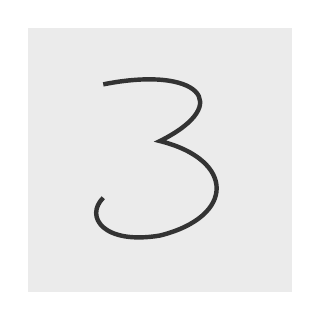
\begin{tikzpicture}[x=0.12cm,y=0.12cm]
                \fill[black!8] (0,0) rectangle (28,28);
                \draw[line width=1.6pt, black!80]
                    (8,22) .. controls (18,24) and (22,20) .. (14,16)
                    .. controls (22,14) and (22,8) .. (14,6)
                    .. controls (8,5) and (6,8) .. (8,10);
            \end{tikzpicture}\\[
0.15em]
            {\scriptsize 自然な「3」：
            $E_\phi$低い\quad$\exp(-E_\phi)$高い}
        \end{column}
        \begin{column}{0.46\textwidth}
            \centering
            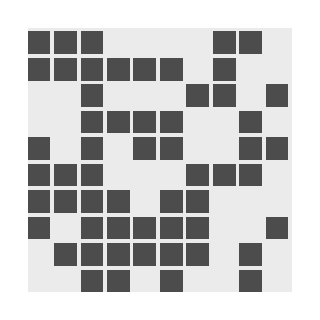
\begin{tikzpicture}[x=0.12cm,y=0.12cm]
                \pgfmathsetseed{3}
                \fill[black!8] (0,0) rectangle (28,28);
                \foreach \i in {0,...,9}{
                    \foreach \j in {0,...,9}{
                        \pgfmathparse{100*rnd}
                        \ifdim\pgfmathresult pt>55pt
                            \fill[black!70]
                                (2.8*\i,2.8*\j) rectangle ++(2.4,2.4);
                        \fi
                    }
                }
            \end{tikzpicture}\\[0.15em]
            {\scriptsize ランダム画素：
            $E_\phi$高い\quad$\exp(-E_\phi)$低い}
        \end{column}
    \end{columns}
    \vspace{0.25em}
    \begin{exampleblock}{読み方}
        よく現れる画像ほどエネルギーを下げ、現れにくい画像ほど上げる。
        だから$p_\phi(\bm{x})\propto\exp(-E_\phi(\bm{x}))$では、
        よく出る画像ほど確率が高くなる。
    \end{exampleblock}
\end{frame}
%=============================================
\assuppl
\begin{frame}{補足：エネルギーを確率密度へ変換する}
    \begin{exampleblock}{エネルギーそのものは確率ではない}
        $E_\phi:\mathbb{R}^{D}\to\mathbb{R}$を、
        $\exp(-E_\phi(\bm{x}))$で正の量に変える。\\
        エネルギーが$1$違うと、$\exp(-E)$は$e$倍になる。
    \end{exampleblock}
    \centering
    \renewcommand{\arraystretch}{1.2}
    \begin{tabular}{ccc}
        \hline
        エネルギー & $\exp(-E)$ & 相対的な密度 \\
        \hline
        $-1$ & $e\approx 2.72$ & 高い \\
        $0$ & $1$ & 中程度 \\
        $1$ & $e^{-1}\approx 0.368$ & 低い \\
        \hline
    \end{tabular}
    \vfill
    \begin{exampleblock}{まだ正規化されていない}
        $\exp(-E_\phi(\bm{x}))$の積分は一般に$1$ではない。
        分配関数$Z_\phi$で割って確率密度にする。
    \end{exampleblock}
\end{frame}
%=============================================
\assuppl
\begin{frame}{補足：分配関数が積分を$1$にする}
    $0<Z_\phi<\infty$を仮定する。
    \begin{align*}
        \int_{\mathbb{R}^{D}}p_\phi(\bm{x})\,d\bm{x}
        &=
        \int_{\mathbb{R}^{D}}
        \frac{\exp\!\bigl(-E_\phi(\bm{x})\bigr)}{Z_\phi}
        \,d\bm{x}\\[4pt]
        &=
        \frac{1}{Z_\phi}
        \int_{\mathbb{R}^{D}}
        \exp\!\bigl(-E_\phi(\bm{x})\bigr)
        \,d\bm{x}\\[4pt]
        &=
        \frac{Z_\phi}{Z_\phi}
        =1.
    \end{align*}
    \begin{exampleblock}{役割}
        分配関数は、非正規化密度を
        積分が$1$の確率密度へ変換する。
    \end{exampleblock}
\end{frame}
%=============================================
\asmain
\begin{frame}{図3.1：学習で密度を上げ下げする}
    \centering
    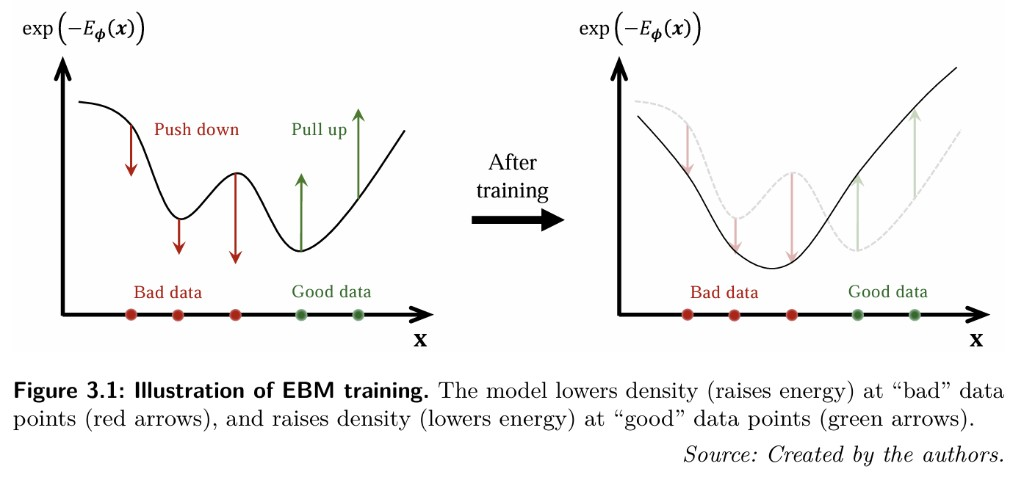
\includegraphics[width=\textwidth,height=0.72\textheight,keepaspectratio]{fig-3-1.jpg}
    \vfill
    赤は密度を下げる方向、緑は上げる方向である。
    右の実線が学習後で、破線は学習前の曲線である。
\end{frame}
%=============================================
\assuppl
\begin{frame}{補足：図3.1は学習前後の比較}
    \begin{columns}[c,onlytextwidth]
        \begin{column}{0.42\textwidth}
            \begin{exampleblock}{学習前}
                \begin{itemize}
                    \item 赤の点にも高い密度
                    \item 緑の点には密度が足りない
                \end{itemize}
            \end{exampleblock}
        \end{column}
        \begin{column}{0.14\textwidth}
            \centering
            {\Large\textcolor{examplecol}{$\longrightarrow$}}\\[0.3em]
            {\footnotesize\bfseries 学習}
        \end{column}
        \begin{column}{0.42\textwidth}
            \begin{exampleblock}{学習後}
                \begin{itemize}
                    \item 赤の近くの密度を\textcolor{alertcol}{\textbf{下げる}}
                    \item 緑の近くの密度を\textcolor{examplecol}{\textbf{上げる}}
                \end{itemize}
            \end{exampleblock}
        \end{column}
    \end{columns}
    \vspace{0.7em}
    \begin{exampleblock}{図の読み方}
        \begin{itemize}
            \item 左図 $\to$ 右図が「学習前 $\to$ 学習後」
            \item 赤の矢印：密度を下げる（エネルギーを上げる）
            \item 緑の矢印：密度を上げる（エネルギーを下げる）
            \item 右図の破線は学習前、実線は学習後
        \end{itemize}
    \end{exampleblock}
\end{frame}
%=============================================
\asmain
\begin{frame}{重要なのはエネルギーの相対値}
    \begin{block}{定数を加えても分布は変わらない}
        すべてのエネルギーに同じ定数を足しても、
        分子と分母が同じ倍率で変わり、確率分布は不変である。
    \end{block}
    \begin{itemize}
        \item エネルギーの絶対値ではなく、点どうしの高低が意味をもつ
        \item ある領域のエネルギーを下げると、その領域の確率は増える
        \item 積分は$1$のままなので、補集合の確率は相対的に減る
    \end{itemize}
    \begin{block}{全体的なトレードオフ}
        確率質量は領域ごとに独立には割り当てられない。
        空間全体で再分配される。
    \end{block}
\end{frame}
%=============================================
\assuppl
\begin{frame}{補足：定数シフトで分布が不変になる}
    \begin{columns}[T,onlytextwidth]
        \begin{column}{0.48\textwidth}
            \begin{exampleblock}{和：エネルギーに定数を足す}
                $E'_\phi(\bm{x})=E_\phi(\bm{x})+c$とする。
                \vspace{-0.3em}
                \begin{align*}
                    p'_\phi(\bm{x})
                    &=
                    \frac{\exp\!\bigl(-(E_\phi(\bm{x})+c)\bigr)}{Z'}\\[2pt]
                    &=
                    \frac{e^{-c}\exp\!\bigl(-E_\phi(\bm{x})\bigr)}{e^{-c}Z_\phi}\\[2pt]
                    &=
                    p_\phi(\bm{x})
                \end{align*}
            \end{exampleblock}
        \end{column}
        \begin{column}{0.48\textwidth}
            \begin{exampleblock}{積：重みに正定数をかける}
                $\tilde{p}'(\bm{x})=a\,\tilde{p}(\bm{x})$（$a>0$）とする。
                \vspace{-0.3em}
                \[
                    \begin{aligned}
                    p'(\bm{x})
                    &=
                    \frac{a\,\tilde{p}(\bm{x})}{\int a\,\tilde{p}(\bm{u})\,d\bm{u}}\\[2pt]
                    &=
                    \frac{\tilde{p}(\bm{x})}{Z}
                    =
                    p(\bm{x})
                    \end{aligned}
                \]
            \end{exampleblock}
        \end{column}
    \end{columns}
    \vspace{0.2em}
    \begin{exampleblock}{読み方}
        和はエネルギーの平行移動、積は非正規化密度の定数倍である。\\
        どちらも分子と分母が同じだけ変わり、分布$p$は不変である。\\
        意味をもつのは絶対値ではなく、点どうしの相対関係である。
    \end{exampleblock}
\end{frame}
%=============================================
\assuppl
\begin{frame}{補足：エネルギーを下げた領域へ質量が移る}
    領域$A$とその補集合$A^{c}$について、
    $P_\phi(A)+P_\phi(A^{c})=1$である。
    $A$のエネルギーだけを$\delta>0$だけ下げると、
    $A$の非正規化密度は$e^{\delta}$倍になる。
    \[
        P'_\phi(A)
        =
        \frac{
        e^{\delta}P_\phi(A)
        }{
        e^{\delta}P_\phi(A)+P_\phi(A^{c})
        }
\]
    $0<P_\phi(A)<1$なら$P'_\phi(A)>P_\phi(A)$。
    \begin{exampleblock}{例}
        $P_\phi(A)$が$0.3$から$0.5$に増えると、
        $P_\phi(A^{c})$は$0.7$から$0.5$へ減る。
        \vspace{0.3em}
        \centering
        \begin{tikzpicture}[x=0.55cm,y=0.55cm,font=\scriptsize]
            \begin{scope}
                \draw[thick] (0,0) rectangle (5.2,3.2);
                \fill[examplecol!35] (1.55,1.6) circle (0.95);
                \draw[examplecol,thick] (1.55,1.6) circle (0.95);
                \node at (1.55,1.6) {$A$};
                \node at (1.55,0.35) {$0.3$};
                \node at (4.0,1.6) {$A^{c}$};
                \node at (4.0,0.9) {$0.7$};
                \node[below] at (2.6,-0.15) {前};
            \end{scope}
            \draw[->,thick] (5.9,1.6) -- (6.7,1.6);
            \begin{scope}[xshift=7.4cm]
                \draw[thick] (0,0) rectangle (5.2,3.2);
                \fill[examplecol!35] (2.1,1.6) circle (1.35);
                \draw[examplecol,thick] (2.1,1.6) circle (1.35);
                \node at (2.1,1.6) {$A$};
                \node at (2.1,0.15) {$0.5$};
                \node at (4.35,2.5) {$A^{c}$};
                \node at (4.35,1.9) {$0.5$};
                \node[below] at (2.6,-0.15) {後};
            \end{scope}
        \end{tikzpicture}
    \end{exampleblock}
\end{frame}
%=============================================
\asmain
\begin{frame}{最尤学習の目的}
    原理上、EBMは最尤推定で学習できる。
    データへの適合と、分布全体の正規化が同時に現れる。
    \[
        \begin{aligned}
        \mathcal{L}_{\mathrm{MLE}}(\phi)
        &=
        \underbrace{
        -\mathbb{E}_{p_{\mathrm{data}}}[E_\phi(\bm{x})]
        }_{\text{実データのエネルギーを下げる}}
        -
        \underbrace{\log Z_\phi}_{\text{大域的な正規化}}
        \end{aligned}
        \tag{3.1.1}
\]
    \begin{block}{二つの項}
        第1項は学習データのエネルギーを下げる。\\
        第2項は、空間全体のエネルギーを無制限には下げさせない。\\
        ⇒最尤推定で見るのは、実データの重みが、全体の重みに対してどれだけ増えたか
    \end{block}
\end{frame}
%=============================================
\assuppl
\begin{frame}{補足：式（3.1.1）の導出}
    \[
        \mathcal{L}_{\mathrm{MLE}}(\phi)
        =
        \mathbb{E}_{p_{\mathrm{data}}(\bm{x})}
        [\log p_\phi(\bm{x})]
\]
    にEBMの密度を代入する。
    \begin{align*}
        \log p_\phi(\bm{x})
        &=
        -E_\phi(\bm{x})-\log Z_\phi,\\[
4pt]
        \mathcal{L}_{\mathrm{MLE}}(\phi)
        &=
        -\mathbb{E}_{p_{\mathrm{data}}}[E_\phi(\bm{x})]
        -\log Z_\phi.
    \end{align*}
    \begin{exampleblock}{第2項の意味}
        ここでの正則化は重み減衰ではない。
        確率分布の正規化から出る項である。
        あらゆる場所のエネルギーを下げると$Z_\phi$が大きくなり、
        $-\log Z_\phi$は小さくなる。
    \end{exampleblock}
\end{frame}
%=============================================
\assuppl
\begin{frame}{補足：AとBだけで見る最尤の二つの項}
    候補は$A,B$の2点だけ、実データは$A$とする。
    重みは$w(\bm{x})=\exp\!\bigl(-E_\phi(\bm{x})\bigr)$、
    確率は$P(A)=\dfrac{w(A)}{w(A)+w(B)}$である。
    \vspace{0.35em}
    \centering
    \renewcommand{\arraystretch}{1.55}
    \begin{tabular}{lccc}
        \hline
        & $w(A)$ & $w(B)$ & $P(A)$ \\
        \hline
        初期 & $1$ & $1$ & $1/2$ \\
        $A$だけ下げる & $2$ & $1$ & $2/3$ \\
        両方上げる & $2$ & $2$ & $2/4=1/2$ \\
        \hline
    \end{tabular}
    \vspace{0.45em}
    \begin{columns}[T,onlytextwidth]
        \begin{column}{0.48\textwidth}
            \begin{exampleblock}{$A$だけ下げる}
                $A$の重みは2倍だが、
                全体も$2\to 3$へ増える。\\
                第1項の改善を第2項が一部打ち消しても、
                合計では$\frac12\to\frac23$へ改善する。
            \end{exampleblock}
        \end{column}
        \begin{column}{0.48\textwidth}
            \begin{exampleblock}{両方を同じだけ}
                両方の重みを$2$にすると、
                $P(A)$は$\frac12$のまま。\\
                二つの変化は完全に打ち消し合う。
            \end{exampleblock}
        \end{column}
    \end{columns}
\end{frame}
%=============================================
\assuppl
\begin{frame}{補足：いつも片方を犠牲にするわけではない}
    $A$のエネルギーを下げながら$B$のエネルギーを上げ、
    全体の重みも減るなら、二つの項はどちらも大きくなり得る。
    \begin{exampleblock}{読み方}
        いつも片方を改善するともう片方が悪化するわけではない。\\
        データの適合（第1項）と正規化（第2項）は、
        状況によって同時に改善し得る。
    \end{exampleblock}
    \begin{exampleblock}{見ているもの}
        最尤推定が見ているのは、
        実データの重みが全体の重みに対してどれだけ増えたかである。
    \end{exampleblock}
\end{frame}
%=============================================
\asmain
\begin{frame}{最尤学習が難しい理由}
    \[
        \mathcal{L}_{\mathrm{MLE}}(\phi)
        =
        -\mathbb{E}_{p_{\mathrm{data}}}[E_\phi(\bm{x})]
        -\log Z_\phi
\]
    高次元では$\log Z_\phi$とその$\phi$勾配を、
    一般には計算できない。
    \[
        \nabla_\phi\log Z_\phi
        =
        -\mathbb{E}_{p_\phi(\bm{x})}
        [\nabla_\phi E_\phi(\bm{x})]
\]
    \begin{block}{必要な期待値が二つある}
        実データについての期待値は学習データから推定できる。
        モデル分布$p_\phi$についての期待値は、
        分布全体の積分または高コストなサンプリングを要する。
    \end{block}
\end{frame}
%=============================================
\assuppl
\begin{frame}{補足：$\log Z_\phi$の勾配}
    微分と積分の交換（優収束定理／Leibniz rule）のもとで、
    \begin{align*}
        \nabla_\phi\log Z_\phi
        &=
        \frac{1}{Z_\phi}
        \nabla_\phi
        \int
        \exp\!\bigl(-E_\phi(\bm{x})\bigr)
        \,d\bm{x}\\[
4pt]
        &=
        \frac{1}{Z_\phi}
        \int
        -\exp\!\bigl(-E_\phi(\bm{x})\bigr)
        \nabla_\phi E_\phi(\bm{x})
        \,d\bm{x}\\[4pt]
        &=
        -\mathbb{E}_{p_\phi}
        [\nabla_\phi E_\phi(\bm{x})].
    \end{align*}
    \begin{exampleblock}{最後の変形}
        $\dfrac{\exp\!\bigl(-E_\phi(\bm{x})\bigr)}{Z_\phi}=p_\phi(\bm{x})$なので、
        積分をモデル分布$p_\phi$の下での期待値と書ける。
    \end{exampleblock}
\end{frame}
%=============================================
\assuppl
\begin{frame}{補足：交換が許される条件}
    $\phi$の近傍で$E_\theta(\bm{x})$が$\theta$について微分可能と仮定する。
    \begin{exampleblock}{十分条件（優収束）}
        近傍のすべての$\theta$に対し、$\theta$に依らない可積分な$g$があり
        \[
            \bigl\|\nabla_\theta\exp\!\bigl(-E_\theta(\bm{x})\bigr)\bigr\|
            \le g(\bm{x}),
            \qquad
            \int g(\bm{x})\,d\bm{x}<\infty
\]
        とする。優収束の対象は、$\phi$と$\phi+h$を含む差分商である。
    \end{exampleblock}
    \begin{exampleblock}{この条件が保証すること}
        $0<Z_\phi<\infty$を仮定する。
        上の条件のもとでは、差分商も同じ$g(\bm{x})$で抑えられるため、
        優収束定理により微分と積分を交換できる。
        また、$\mathbb{E}_{p_\phi}[\|\nabla_\phi E_\phi(\bm{x})\|]<\infty$も従う。
    \end{exampleblock}
\end{frame}
%=============================================
\assuppl
\begin{frame}{補足：最尤勾配は二つの期待値の差}
    \[
        \resizebox{0.98\textwidth}{!}{$
        \nabla_\phi\mathcal{L}_{\mathrm{MLE}}(\phi)
        =
        -\mathbb{E}_{p_{\mathrm{data}}}
        [\nabla_\phi E_\phi(\bm{x})]
        +
        \mathbb{E}_{p_\phi}
        [\nabla_\phi E_\phi(\bm{x})]
        $}
\]
    \begin{exampleblock}{読み方}
        データ上ではエネルギーを下げる方向へ更新し、
        モデルが今確率を置いている場所では
        エネルギーを上げる方向へ更新する。
    \end{exampleblock}
    \begin{exampleblock}{回避の方向}
        コントラスティブ・ダイバージェンスは
        分配関数の項を近似する。
        スコアマッチングは、その項の計算自体を避ける。
    \end{exampleblock}
\end{frame}
%=============================================
\asmain
\begin{frame}{3.1.1 のまとめ}
    \begin{itemize}
        \item EBMは$E_\phi$と分配関数$Z_\phi$で密度を定義する
        \item 意味をもつのはエネルギーの相対値であり、
        確率質量は空間全体で再分配される
        \item 最尤勾配にはモデル分布$p_\phi$についての期待値が必要で、
        高次元では計算が困難である
    \end{itemize}
    \begin{block}{次}
        3.1.2では、分配関数を含まないスコアを導入する。
    \end{block}
\end{frame}
%=============================================
\section{3.1.2 スコア関数}
\asmain
\begin{frame}{区切り：3.1.2 スコア関数}
    \tableofcontents[currentsection]
\end{frame}
%=============================================
\asmain
\begin{frame}{3.1.2 スコアとは何か}
    $\mathbb{R}^{D}$上の確率密度$p(\bm{x})$に対し、
    スコアは対数密度の勾配である。

    \vspace{0.15em}
    \begin{columns}[c,onlytextwidth]
        \begin{column}{0.34\textwidth}
            \centering
            \[
                s(\bm{x})
                :=
                \nabla_{\bm{x}}\log p(\bm{x})
            \]
            \[
                s:\mathbb{R}^{D}\to\mathbb{R}^{D}
            \]
        \end{column}
        \begin{column}{0.64\textwidth}
            \centering
            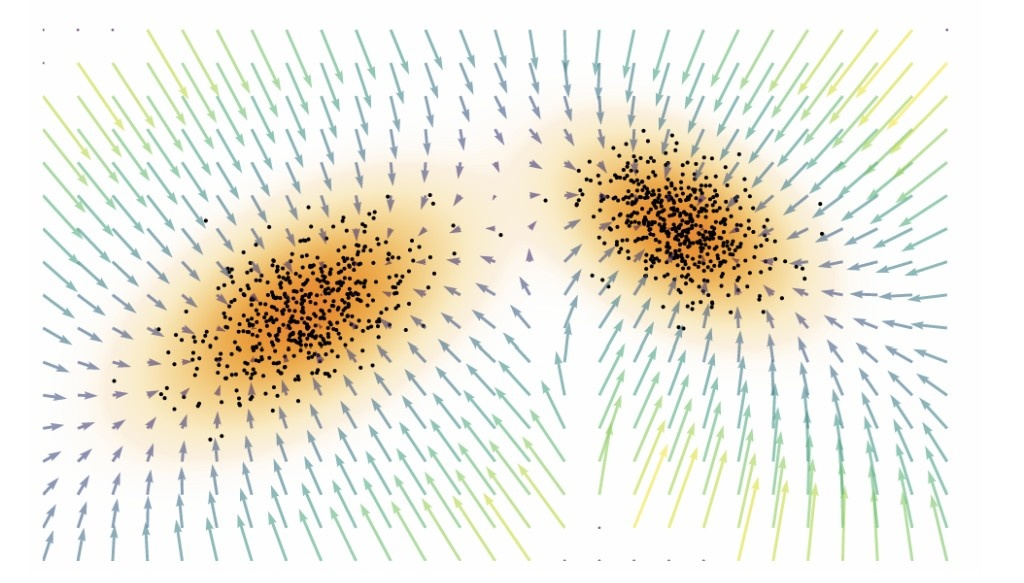
\includegraphics[width=\linewidth,height=0.47\textheight,keepaspectratio]{fig-3-2-nocaption.jpg}\\[0.15em]
            {\footnotesize 図3.2：矢印はスコアで、近い山の中心を向く。}
        \end{column}
    \end{columns}

    \vfill
    \begin{block}{直感}
        スコアは、確率密度がより高い領域へ向かう
        方向を示すベクトル場である。
        密度の値そのものではなく、
        局所的にどちらへ進めば密度が増えるかを与える。
    \end{block}
\end{frame}
%=============================================
\assuppl
\begin{frame}{イメージで理解する：データ分布からスコアへ}
    データ点の分布から、密度の山とスコアの矢印がどう決まるかを
    イメージで確認できる。
    \begin{exampleblock}{インタラクティブな可視化}
        データの配置 $\to$ 密度の形 $\to$ スコアベクトル場、
        という流れを追いながら、
        「近い山の中心を向く」意味を掴める。
        \vspace{0.4em}
        \begin{center}
            \href{https://ebm-data-to-score.intactspoon4.chatgpt.site/space.html?dim=3}
            {\scriptsize\texttt{https://ebm-data-to-score.intactspoon4.chatgpt.site/space.html?dim=3}}
        \end{center}
    \end{exampleblock}
\end{frame}
%=============================================
\assuppl
\begin{frame}{補足：スコアの成分と相対変化率}
    \[
        s(\bm{x})
        =
        \begin{pmatrix}
            \partial_{x_1}\log p(\bm{x})\\
            \vdots\\
            \partial_{x_D}\log p(\bm{x})
        \end{pmatrix}
\]
    入力が$D$次元なら、スコアも$D$次元である。
    \[
        \nabla_{\bm{x}}\log p(\bm{x})
        =
        \frac{\nabla_{\bm{x}}p(\bm{x})}{p(\bm{x})}
\]
    \begin{exampleblock}{定義される場所}
        スコアは密度の絶対的な変化量ではなく、
        その点の密度に対する相対的な変化率である。
        $p(\bm{x})>0$で微分可能な領域で定義される。
    \end{exampleblock}
\end{frame}
%=============================================
\assuppl
\begin{frame}{補足：標準正規分布では中心を向く}
    \begin{columns}[c,onlytextwidth]
        \begin{column}{0.34\textwidth}
            \footnotesize
            \begin{align*}
                p(x)
                &=
                \tfrac{1}{\sqrt{2\pi}}
                e^{-x^2/2}\\[2pt]
                \log p(x)
                &=
                -\tfrac12\log(2\pi)
                -\tfrac{x^2}{2}\\[2pt]
                s(x)
                &=
                -x
            \end{align*}
            \begin{exampleblock}{読み方}
                $x<0\Rightarrow s>0$（右へ）\\
                $x>0\Rightarrow s<0$（左へ）\\
                どちらも密度最大の$0$へ。
            \end{exampleblock}
            \vspace{0.3em}
            {\scriptsize 多峰なら局所的な増加方向で、大域最大とは限らない。}
        \end{column}
        \begin{column}{0.64\textwidth}
            \centering
            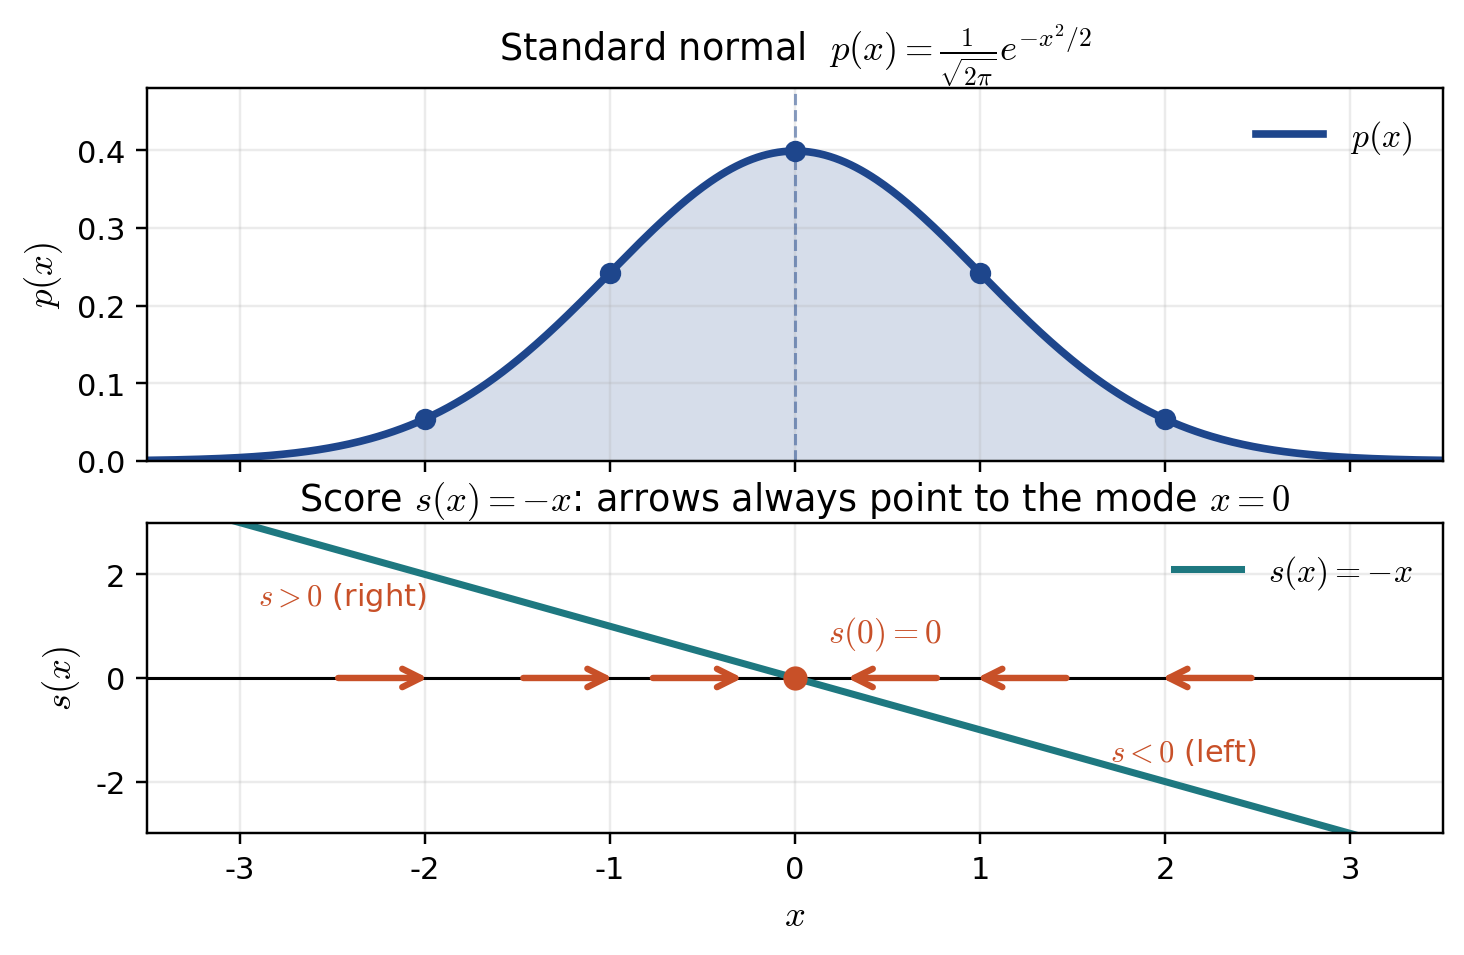
\includegraphics[width=\linewidth,height=0.72\textheight,keepaspectratio]{score-standard-normal.png}
        \end{column}
    \end{columns}
\end{frame}
%=============================================
\asmain
\begin{frame}{EBMのスコアから分配関数が消える}
    \[
        p_\phi(\bm{x})
        =
        \frac{\exp\!\bigl(-E_\phi(\bm{x})\bigr)}{Z_\phi}
\]
    の対数勾配は
    \[
        s_\phi(\bm{x})
        =
        -\nabla_{\bm{x}}E_\phi(\bm{x})
\]
    \begin{block}{二つの微分を区別する}
        $\nabla_\phi\log Z_\phi$は一般に計算が困難である。
        $\nabla_{\bm{x}}\log Z_\phi=0$であり、
        入力で微分すると分配関数は残らない。
    \end{block}
    エネルギーが下がる方向と、密度が増える方向は一致する。
\end{frame}
%=============================================
\assuppl
\begin{frame}{補足：EBMのスコアの計算}
    \begin{align*}
        s_\phi(\bm{x})
        &=
        \nabla_{\bm{x}}\log p_\phi(\bm{x})\\
        &=
        \nabla_{\bm{x}}
        \bigl[-E_\phi(\bm{x})-\log Z_\phi\bigr]\\
        &=
        -\nabla_{\bm{x}}E_\phi(\bm{x}).
    \end{align*}
    \begin{exampleblock}{非正規化密度だけでも同じ}
        $\tilde{p}_\phi(\bm{x})=\exp(-E_\phi(\bm{x}))$とすると、
        \[
            \nabla_{\bm{x}}\log p_\phi(\bm{x})
            =
            \nabla_{\bm{x}}\log\tilde{p}_\phi(\bm{x}).
\]
        正規化定数を計算しなくても、
        正規化後の密度のスコアが正確に得られる。
    \end{exampleblock}
\end{frame}
%=============================================
\assuppl
\begin{frame}{補足：スコアの方向に進むだけでは不十分}
    \begin{exampleblock}{ベクトル場の意味}
        二次元なら、各点で
        \[
            s(\bm{x})
            =
            \begin{pmatrix}
                \partial_{x_1}\log p(\bm{x})\\
                \partial_{x_2}\log p(\bm{x})
            \end{pmatrix}
\]
        を返す。これは、その点で密度が最も急に増える方向である。
    \end{exampleblock}
    \begin{exampleblock}{サンプリングとの違い}
        矢印に沿って進み続けるだけでは、
        分布全体からのサンプルにはならない。
        山の頂上へ吸い寄せられる。
        分布に従うサンプリングには、
        後のランジュバン動力学のように確率的なノイズも要る。
    \end{exampleblock}
\end{frame}
%=============================================
\asmain
\begin{frame}{正規化定数に依存しない}
    多くの分布は非正規化密度$\tilde{p}(\bm{x})$で定義される。
    \[
        p(\bm{x})
        =
        \frac{\tilde{p}(\bm{x})}{Z},
        \qquad
        Z=\int\tilde{p}(\bm{x})\,d\bm{x}
\]
    $Z$は$\bm{x}$に依らないので、
    \[
        \begin{aligned}
        \nabla_{\bm{x}}\log p(\bm{x})
        &=
        \nabla_{\bm{x}}\log\tilde{p}(\bm{x})
        -
        \underbrace{\nabla_{\bm{x}}\log Z}_{=0}\\
        &=
        \nabla_{\bm{x}}\log\tilde{p}(\bm{x})
        \end{aligned}
        \tag{3.1.2}
    \]
    \begin{block}{利点}
        スコアを扱うことで、分配関数の計算を避けられる。
        未知のスコアをどう推定するかは、次のスコアマッチングの問題である。
    \end{block}
\end{frame}
%=============================================
\asmain
\begin{frame}{スコアは分布を定数を除いて決める}
    スコアは対数密度の勾配なので、基準点$\bm{x}_0$からの積分で
    対数密度を復元できる。
    \[
        \resizebox{0.98\textwidth}{!}{$
        \log p(\bm{x})
        =
        \log p(\bm{x}_0)
        +
        \displaystyle\int_0^1
        s\!\left(\bm{x}_0+t(\bm{x}-\bm{x}_0)\right)^{\!\top}
        (\bm{x}-\bm{x}_0)
        \,dt
        $}
\]
    \begin{block}{同等の表現力}
        スコアが正確にわかれば、適切な条件のもとで
        確率密度$p(\bm{x})$も一意に決められる。\\
        密度そのものをモデル化する方法と、
        スコアをモデル化する方法は、理論上同じ分布を表現できる。\\
        学習とサンプリングでは、密度そのものより扱いやすいことが多い。
    \end{block}
\end{frame}
%=============================================
\assuppl
\begin{frame}{補足：基準点からの変化量を足す}
    前の式は、基準点$\bm{x}_0$での$\log p(\bm{x}_0)$に、
    $\bm{x}_0$から$\bm{x}$までの変化量を足すと$\log p(\bm{x})$が求まる、
    ことを表す。
    \[
        s(\bm{x})=\nabla_{\bm{x}}\log p(\bm{x})
    \]
    経路上で$p>0$かつ微分可能とする。
    \begin{exampleblock}{直線経路}
        \[
            \bm{z}(t)=\bm{x}_0+t(\bm{x}-\bm{x}_0)
            \qquad(t=0\Rightarrow\bm{x}_0,\;\; t=1\Rightarrow\bm{x})
        \]
        知りたいのは、移動に伴う$\log p(\bm{z}(t))$の変化である。
    \end{exampleblock}
\end{frame}
%=============================================
\assuppl
\begin{frame}{補足：積分の中身は$\log p$の$t$微分}
    合成関数の微分より
    \[
        \frac{d}{dt}\log p(\bm{z}(t))
        =
        \underbrace{s(\bm{z}(t))^{\top}}_{\text{その位置のスコア}}
        \underbrace{(\bm{x}-\bm{x}_0)}_{d\bm{z}/dt}
    \]
    つまり、元の式の積分の中身は$\log p$の$t$に関する微分である。
    \begin{exampleblock}{転置と内積}
        「その方向への変化のしやすさ$\times$その方向への移動量」を
        座標ごとに計算し、足し合わせている。
        二次元なら
        \[
            s(\bm{z})^{\top}(\bm{x}-\bm{x}_0)
            =
            s_1(\bm{z})(x_1-x_{0,1})
            +
            s_2(\bm{z})(x_2-x_{0,2})
        \]
    \end{exampleblock}
\end{frame}
%=============================================
\assuppl
\begin{frame}{補足：微分を積分すると変化量が求まる}
    $t=0$から$1$まで積分する。
    \begin{align*}
        \int_0^1
        s(\bm{z}(t))^{\top}(\bm{x}-\bm{x}_0)\,dt
        &=
        \int_0^1\frac{d}{dt}\log p(\bm{z}(t))\,dt\\
        &=
        \log p(\bm{x})-\log p(\bm{x}_0)
    \end{align*}
    $\log p(\bm{x}_0)$を移項すれば、本文の復元式になる。
    \begin{exampleblock}{要点}
        「微分を積分すると変化量が求まる」を、
        多変数の$\log p$に使った式である。\\
        スコアから求まるのはまず差$\log p(\bm{x})-\log p(\bm{x}_0)$で、
        値そのものには基準の値も要る。
    \end{exampleblock}
\end{frame}
%=============================================
\assuppl
\begin{frame}{補足：積分定数は正規化で決まる}
    スコアは$\log p$の微分なので、積分すると
    \[
        \log p(\bm{x})=F(\bm{x})+C
    \]
    となる。$F$はスコアを積分した関数、$C$は$\bm{x}$に依らない定数
    （普通の不定積分の定数と同じ）。
    両辺の指数を取ると
    \[
        p(\bm{x})=e^{F(\bm{x})+C}=e^{C}\,e^{F(\bm{x})}
    \]
    まだ決まっていないのは、密度全体に掛かる定数$e^{C}$である。
\end{frame}
%=============================================
\assuppl
\begin{frame}{補足：正規化で$e^{C}$を決める}
    正規化条件$\displaystyle\int p(\bm{x})\,d\bm{x}=1$に代入する。
    \[
        \int e^{C}\,e^{F(\bm{x})}\,d\bm{x}=1
    \]
    $e^{C}$は$\bm{x}$に依らないので外に出せる。
    \[
        e^{C}\int e^{F(\bm{x})}\,d\bm{x}=1
        \qquad\Rightarrow\qquad
        e^{C}
        =
        \frac{1}{\int e^{F(\bm{x})}\,d\bm{x}}
        =
        \Bigl(\int e^{F(\bm{x})}\,d\bm{x}\Bigr)^{-1}
    \]
    したがって
    \[
        p(\bm{x})
        =
        \frac{e^{F(\bm{x})}}{\int e^{F(\bm{u})}\,d\bm{u}}
    \]
    \begin{exampleblock}{読み方}
        スコアの積分で得た$e^{F}$を、全体の積分値で割って
        積分が$1$になるようにしている。
    \end{exampleblock}
\end{frame}
%=============================================
\assuppl
\begin{frame}{補足：一意性と同等の表現力}
    \begin{exampleblock}{一意性と同等の表現力}
        連結領域上で正の正規化可能密度があり、
        スコアが全域で正確なら$p$は一意に定まる。\\
        密度そのものをモデル化する方法と、
        スコアをモデル化する方法は、理論上同じ分布を表せる
        （同等の表現力をもつ）。\\
        ただし任意のベクトル場がスコアになるわけではなく、
        対数密度の勾配として積分可能である必要がある。
    \end{exampleblock}
    \begin{exampleblock}{理論と計算}
        復元できることと、高次元で正規化積分を
        効率よく計算できることは別である。
    \end{exampleblock}
\end{frame}
%=============================================
\asmain
\begin{frame}{3.1.2 のまとめ}
    \begin{itemize}
        \item スコア$s(\bm{x})=\nabla_{\bm{x}}\log p(\bm{x})$は
        密度が増える方向を与える
        \item EBMのスコアは$s_\phi=-\nabla_{\bm{x}}E_\phi$となり、
        分配関数$Z_\phi$を含まない
        \item スコアが正確なら、適切な条件のもとで$p$は一意に決まる
        （密度モデルと同等の表現力）
    \end{itemize}
    \begin{block}{次}
        3.1.3では、未知のデータ分布のスコアを
        どう学習するかを扱う。
    \end{block}
\end{frame}
%=============================================
\section{3.1.3 スコアマッチング}
\asmain
\begin{frame}{区切り：3.1.3 スコアマッチング}
    \tableofcontents[currentsection]
\end{frame}
%=============================================
\asmain
\begin{frame}{3.1.3 スコアを合わせてEBMを学習する}
    モデルのスコアはエネルギーだけで書け、$Z_\phi$に依らない。
    \[
        \nabla_{\bm{x}}\log p_\phi(\bm{x})
        =
        -\nabla_{\bm{x}}E_\phi(\bm{x})
\]
    スコアマッチングは、正規化密度を直接合わせる代わりに、\\
    モデルのスコアをデータ分布のスコアへ近づける。
    \[
        \mathcal{L}_{\mathrm{SM}}(\phi)
        =
        \frac12
        \mathbb{E}_{p_{\mathrm{data}}}
        \left[
        \left\|
        \nabla_{\bm{x}}\log p_\phi
        -
        \nabla_{\bm{x}}\log p_{\mathrm{data}}
        \right\|_2^2
        \right]
        \tag{3.1.3}
\]
    \footnotesize
    Hyv\"{a}rinen and Dayan (2005)
\end{frame}
%=============================================
\asmain
\begin{frame}{データスコアを消した等価な損失}
    部分積分により、エネルギーとその導関数だけの形に書ける。
    \[
        \resizebox{0.98\textwidth}{!}{$
        \mathcal{L}_{\mathrm{SM}}(\phi)
        =
        \mathbb{E}_{p_{\mathrm{data}}}
        \left[
        -\operatorname{Tr}\!\left(\nabla_{\bm{x}}^{2}E_\phi(\bm{x})\right)
        +
        \frac12
        \left\|\nabla_{\bm{x}}E_\phi(\bm{x})\right\|_2^2
        \right]
        +C
        $}
\]
    $C$は$\phi$に依らない。$\nabla_{\bm{x}}^{2}E_\phi$はヘッセ行列である。
    \begin{block}{利点と欠点}
        分配関数も、学習中のモデルからのサンプリングも要らない。
        代わりに二階微分、正確にはヘッセ行列のトレースが必要で、
        コストは入力次元$D$とともに増える。
    \end{block}
\end{frame}
%=============================================
\assuppl
\begin{frame}{補足：合わせたい二つのスコア}
    \begin{exampleblock}{モデルとデータ}
        \[
            s_\phi(\bm{x})
            =
            \nabla_{\bm{x}}\log p_\phi(\bm{x}),
            \qquad
            s_{\mathrm{data}}(\bm{x})
            =
            \nabla_{\bm{x}}\log p_{\mathrm{data}}(\bm{x})
\]
        学習は$s_\phi(\bm{x})\approx s_{\mathrm{data}}(\bm{x})$を目指す。
    \end{exampleblock}
    \begin{exampleblock}{直接は使えない}
        $p_{\mathrm{data}}$は未知なので、
        $s_{\mathrm{data}}$も計算できない。
        損失から未知のスコアを消去する必要がある。
    \end{exampleblock}
\end{frame}
%=============================================
\assuppl
\begin{frame}{補足：二乗を三つの項に分ける}
    \[
        \|s_\phi-s_{\mathrm{data}}\|_2^2
        =
        \|s_\phi\|_2^2
        -2s_\phi^{\top}s_{\mathrm{data}}
        +\|s_{\mathrm{data}}\|_2^2
\]
    したがって
    \[
        \mathcal{L}_{\mathrm{SM}}
        =
        \frac12\mathbb{E}[\|s_\phi\|_2^2]
        -
        \mathbb{E}[s_\phi^{\top}s_{\mathrm{data}}]
        +C.
\]
    \begin{exampleblock}{定数}
        \[
            C
            =
            \frac12
            \mathbb{E}_{p_{\mathrm{data}}}
            [\|s_{\mathrm{data}}\|_2^2]
\]
        は$\phi$に依らないので、最適化には影響しない。
    \end{exampleblock}
\end{frame}
%=============================================
\assuppl
\begin{frame}{補足：未知のスコアを密度の勾配に書き換える}
    \[
        \mathbb{E}[s_\phi^{\top}s_{\mathrm{data}}]
        =
        \int
        p_{\mathrm{data}}(\bm{x})\,
        s_\phi(\bm{x})^{\top}
        \nabla_{\bm{x}}\log p_{\mathrm{data}}(\bm{x})
        \,d\bm{x}
\]
    \[
        \nabla_{\bm{x}}\log p_{\mathrm{data}}
        =
        \frac{\nabla_{\bm{x}}p_{\mathrm{data}}}{p_{\mathrm{data}}}
\]
    を代入すると$p_{\mathrm{data}}$が約分され、
    \[
        \int
        s_\phi(\bm{x})^{\top}
        \nabla_{\bm{x}}p_{\mathrm{data}}(\bm{x})
        \,d\bm{x}.
\]
\end{frame}
%=============================================
\assuppl
\begin{frame}{補足：部分積分で発散になる}
    境界項が消える正則性を仮定すると、
    \[
        \int
        s_\phi^{\top}\nabla_{\bm{x}}p_{\mathrm{data}}
        \,d\bm{x}
        =
        -\int
        p_{\mathrm{data}}\,
        \nabla_{\bm{x}}\cdot s_\phi
        \,d\bm{x}.
\]
    発散は各成分の偏微分の和である。
    \[
        \nabla_{\bm{x}}\cdot s_\phi(\bm{x})
        =
        \sum_{i=1}^{D}
        \frac{\partial s_{\phi,i}(\bm{x})}{\partial x_i}
\]
    \[
        \mathbb{E}[s_\phi^{\top}s_{\mathrm{data}}]
        =
        -\mathbb{E}[\nabla_{\bm{x}}\cdot s_\phi]
\]
    未知の$s_{\mathrm{data}}$は、モデルのスコアの発散に置き換わる。
\end{frame}
%=============================================
\assuppl
\begin{frame}{補足：エネルギーとヘッセ行列のトレース}
    発散の形に戻すと
    \[
        \mathcal{L}_{\mathrm{SM}}
        =
        \mathbb{E}
        \left[
        \nabla_{\bm{x}}\cdot s_\phi
        +
        \frac12\|s_\phi\|_2^2
        \right]
        +C.
\]
    $s_\phi=-\nabla_{\bm{x}}E_\phi$より
    \[
        \nabla_{\bm{x}}\cdot s_\phi
        =
        -\sum_{i=1}^{D}
        \frac{\partial^{2}E_\phi}{\partial x_i^{2}}
        =
        -\operatorname{Tr}(\nabla_{\bm{x}}^{2}E_\phi).
\]
    これが本文の損失である。
    必要なのはヘッセ行列の全成分ではなく、対角和だけである。
\end{frame}
%=============================================
\assuppl
\begin{frame}{補足：ヘッセ行列とトレース}
    ヘッセ行列は、スカラー関数の二階偏微分を並べた行列である。
    二次元では
    \[
        \nabla_{\bm{x}}^{2}E_\phi
        =
        \begin{pmatrix}
            \partial_{x_1}^{2}E_\phi & \partial_{x_1}\partial_{x_2}E_\phi\\
            \partial_{x_2}\partial_{x_1}E_\phi & \partial_{x_2}^{2}E_\phi
        \end{pmatrix}.
\]
    トレースは対角成分の和なので、
    \[
        \operatorname{Tr}(\nabla_{\bm{x}}^{2}E_\phi)
        =
        \partial_{x_1}^{2}E_\phi
        +
        \partial_{x_2}^{2}E_\phi.
\]
    \begin{exampleblock}{計算上の課題}
        対角和だけでも、各座標の二階微分を集める必要がある。
        $D$が大きいほど厳密な計算は重くなる。
        本章の後半で、この二階微分を避ける方法を扱う。
    \end{exampleblock}
\end{frame}
%=============================================
\assuppl
\begin{frame}{補足：最尤推定とスコアマッチング}
    \centering
    \footnotesize
    \renewcommand{\arraystretch}{1.25}
    \begin{tabular}{|p{0.22\textwidth}|p{0.34\textwidth}|p{0.34\textwidth}|}
        \hline
        & 最尤推定 & スコアマッチング \\
        \hline
        学習目的 & 対数尤度を最大化 & スコアを一致させる \\
        \hline
        分配関数 & 勾配に残る & 不要 \\
        \hline
        モデルからのサンプル & 勾配の近似で要ることが多い & 基本形では不要 \\
        \hline
        主な困難 & モデル分布の期待値 & 二階微分 \\
        \hline
    \end{tabular}
    \vfill
    \normalsize
    \begin{exampleblock}{共通点と違い}
        どちらもモデルをデータ分布へ近づける。
        スコアマッチングが比べるのは密度の値ではなく、
        各点での対数密度の勾配である。
    \end{exampleblock}
\end{frame}
%=============================================
\asmain
\begin{frame}{3.1.3 のまとめ}
    \begin{itemize}
        \item スコアマッチングは、密度ではなくスコアを一致させてEBMを学習する
        \item 部分積分により、未知の$s_{\mathrm{data}}$は
        エネルギーとその二階微分に置き換わる
        \item 分配関数は不要だが、ヘッセ行列のトレースが必要になる
    \end{itemize}
    \begin{block}{次}
        3.1.4では、学習したスコアからサンプルを得る
        ランジュバン動力学を扱う。
    \end{block}
\end{frame}
%=============================================
\section{3.1.4 ランジュバン動力学}
\asmain
\begin{frame}{区切り：3.1.4 ランジュバン動力学}
    \tableofcontents[currentsection]
\end{frame}
%=============================================
\assuppl
\begin{frame}{イメージで理解する：ランジュバン動力学}
    式に入る前に、空間上での動きのイメージを見ておくとわかりやすい。
    \begin{exampleblock}{インタラクティブな可視化}
        スコア（エネルギーの勾配）に沿った移動と、
        ノイズによるゆらぎが合わさる様子を確認できる。
        \vspace{0.4em}
        \begin{center}
            \href{https://ebm-space-motion.intactspoon4.chatgpt.site/}
            {\small\texttt{https://ebm-space-motion.intactspoon4.chatgpt.site/}}
        \end{center}
    \end{exampleblock}
\end{frame}
%=============================================
\asmain
\begin{frame}{離散時間のランジュバン更新}
    EBMからのサンプリングは、ランジュバン動力学で行える。
    \[
        \bm{x}_{n+1}
        =
        \bm{x}_n
        -\eta\nabla_{\bm{x}}E_\phi(\bm{x}_n)
        +\sqrt{2\eta}\,\bm{\epsilon}_n
        \tag{3.1.4}
\]
    $\bm{x}_0$は適当な分布、多くはガウス分布から引く。
    $\eta>0$:ステップ幅、$\bm{\epsilon}_n\sim\mathcal{N}(\bm{0},\bm{I})$\\
    スコア$\nabla_{\bm{x}}\log p_\phi=-\nabla_{\bm{x}}E_\phi$で書き換えると、\\
    \[
        \bm{x}_{n+1}
        =
        \bm{x}_n
        +\eta\nabla_{\bm{x}}\log p_\phi(\bm{x}_n)
        +\sqrt{2\eta}\,\bm{\epsilon}_n
        \tag{3.1.5}
\]
\end{frame}
%=============================================
\asmain
\begin{frame}{連続時間では確率微分方程式になる}
    $\eta\to 0$とすると、更新は次のSDEに収束する。
    \[
        d\bm{x}(t)
        =
        \nabla_{\bm{x}}\log p_\phi(\bm{x}(t))\,dt
        +
        \sqrt{2}\,d\bm{w}(t)
        \tag{3.1.6}
\]
    $\bm{w}(t)$は標準ブラウン運動である。
    式（3.1.4）は、このSDEのオイラー・丸山法による離散化である。
    \begin{block}{定常分布}
        $E_\phi$が十分滑らかで、サンプルが無限遠へ逃げないとき、
        $t\to\infty$で$\bm{x}(t)$の分布は\\$p_\phi$へ収束する。
        追加条件のもとでは、収束は指数的になり得る。
    \end{block}
\end{frame}
%=============================================
\assuppl
\begin{frame}{補足：更新則の三つの部分}
    \[
        \bm{x}_{n+1}
        =
        \bm{x}_n
        -\eta\nabla_{\bm{x}}E_\phi(\bm{x}_n)
        +\sqrt{2\eta}\,\bm{\epsilon}_n
\]
    \begin{exampleblock}{エネルギーを下げる項}
        $-\eta\nabla_{\bm{x}}E_\phi$は、エネルギーが増える方向の逆へ進む。
        エネルギーが低い場所は密度が高いので、
        この項は密度が高い方向への勾配降下である。
    \end{exampleblock}
    \begin{exampleblock}{ノイズ項}
        $\sqrt{2\eta}\,\bm{\epsilon}_n\sim\mathcal{N}(\bm{0},2\eta\bm{I})$。
        勾配だけでは局所的な極小に止まり得る。
        ノイズは他の領域を探索する余地を作るが、
        離れた峰のあいだを必ず効率よく越えられるわけではない。
    \end{exampleblock}
\end{frame}
%=============================================
\assuppl
\begin{frame}{補足：ノイズ係数が$\sqrt{2\eta}$になる理由}
    連続時間の式を幅$\eta$で離散化する。
    \[
        \bm{x}(t+\eta)-\bm{x}(t)
        \approx
        \eta\,s_\phi(\bm{x}(t))
        +
        \sqrt{2}\,\bigl(\bm{w}(t+\eta)-\bm{w}(t)\bigr)
\]
    ブラウン運動の増分は$\mathcal{N}(\bm{0},\eta\bm{I})$なので、
    \[
        \bm{w}(t+\eta)-\bm{w}(t)
        \overset{d}{=}
        \sqrt{\eta}\,\bm{\epsilon}_n.
\]
    したがってノイズ項は$\sqrt{2}\sqrt{\eta}\,\bm{\epsilon}_n=\sqrt{2\eta}\,\bm{\epsilon}_n$。
    \begin{exampleblock}{別の係数}
        $\bm{x}+\frac{\eta}{2}s_\phi+\sqrt{\eta}\,\bm{\epsilon}$
        もよく使う形である。
        違いは時間の尺度の取り方であり、同じ動力学の別表記である。
    \end{exampleblock}
\end{frame}
%=============================================
\assuppl
\begin{frame}{補足：ドリフトと拡散}
    \[
        d\bm{x}(t)
        =
        \underbrace{s_\phi(\bm{x}(t))\,dt}_{\text{ドリフト}}
        +
        \underbrace{\sqrt{2}\,d\bm{w}(t)}_{\text{拡散}}
\]
    \begin{exampleblock}{二つの働き}
        ドリフトはスコアに従い、密度が高い方向へ動かす。
        拡散はブラウン運動によるランダムな揺れである。
    \end{exampleblock}
    \begin{exampleblock}{通常の微分との違い}
        ブラウン運動の経路は、通常の意味ではほとんど確実に微分できない。
        $d\bm{w}(t)$は普通の微小変化ではなく、確率積分で定義される。
    \end{exampleblock}
\end{frame}
%=============================================
\asmain
\begin{frame}{図3.3：スコアに沿った確率的な軌跡}
    \centering
    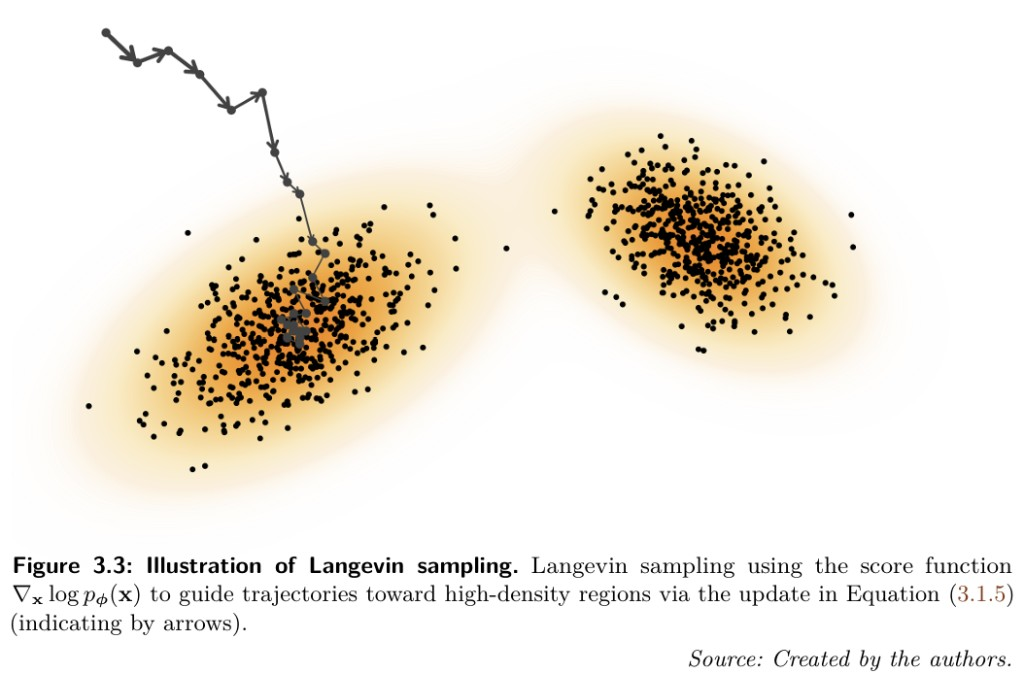
\includegraphics[width=\textwidth,height=0.78\textheight,keepaspectratio]{fig-3-3.jpg}
    \vfill
    式（3.1.5）の更新で、軌跡は左の高密度領域へ入る。右の山へは移っていない。
\end{frame}
%=============================================
\assuppl
\begin{frame}{補足：目標分布が定常分布になる}
    時刻$t$の密度を$q_t$とすると、適切な条件で
    \[
        \partial_t q_t
        =
        -\nabla_{\bm{x}}\cdot
        \bigl(q_t\nabla_{\bm{x}}\log p_\phi\bigr)
        +\Delta q_t.
\]
    $q_t=p_\phi$を代入すると、
    $p_\phi\nabla_{\bm{x}}\log p_\phi=\nabla_{\bm{x}}p_\phi$より
    \[
        \partial_t q_t
        =
        -\Delta p_\phi+\Delta p_\phi
        =0.
\]
    \begin{exampleblock}{読み方と限界}
        $p_\phi$は時間的に変化しない定常分布である。
        初期分布からの収束には、エルゴード性などの追加条件が要る。
        有限の$\eta$では離散化誤差があり、
        離散連鎖の定常分布は厳密には$p_\phi$と一致しない。
    \end{exampleblock}
\end{frame}
%=============================================
\asmain
\begin{frame}{なぜランジュバン動力学なのか}
    エネルギーの勾配だけに従う決定論的な運動は
    \[
        d\bm{x}(t)
        =
        -\nabla_{\bm{x}}E_\phi(\bm{x}(t))\,dt
\]
    であり、局所的な極小へ向かう。
    そこにノイズを加えると
    \[
        d\bm{x}(t)
        =
        -\nabla_{\bm{x}}E_\phi(\bm{x}(t))\,dt
        +
        \sqrt{2}\,d\bm{w}(t)
\]
    となる。適切な条件のもとで、定常分布は
    $p_\phi(\bm{x})\propto e^{-E_\phi(\bm{x})}$である。
    \begin{block}{EBMでの使い道}
        分配関数を計算せず、エネルギーの勾配だけで
        $p_\phi$からのサンプルを近似できる。
    \end{block}
\end{frame}
%=============================================
\assuppl
\begin{frame}{補足：勾配は力、ただし過減衰の運動}
    力は$F(\bm{x})=-\nabla_{\bm{x}}E(\bm{x})$である。
    $E(x)=\frac12 x^2$なら$F(x)=-x$で、粒子は原点へ向かう。
    \begin{exampleblock}{本文のODEとの違い}
        $d\bm{x}=-\nabla_{\bm{x}}E_\phi\,dt$は、
        ニュートンの$m\ddot{\bm{x}}=F$そのものではない。
        慣性を無視した、過減衰系の一次の運動である。
    \end{exampleblock}
    この流れに沿うと
    \[
        \frac{d}{dt}E_\phi(\bm{x}(t))
        =
        -\|\nabla_{\bm{x}}E_\phi\|_2^2
        \le 0.
\]
    エネルギーは増えない。別の谷へ行くには、
    一時的にエネルギーを上げる必要があり、決定論だけでは足りない。
\end{frame}
%=============================================
\assuppl
\begin{frame}{補足：$\sqrt{2}$は定常性から決まる}
    一般のSDE
    $d\bm{x}=b\,dt+\sigma\,d\bm{w}$の密度は
    \[
        \partial_t\rho
        =
        -\nabla\cdot(b\rho)
        +\frac{\sigma^2}{2}\Delta\rho.
\]
    $b=\nabla_{\bm{x}}\log p_\phi$、$\rho=p_\phi$とすると
    \[
        \partial_t\rho
        =
        \left(\frac{\sigma^2}{2}-1\right)\Delta p_\phi.
\]
    これが一般の分布で$0$になるには$\sigma=\sqrt{2}$。
    \begin{exampleblock}{脚注の意味}
        $\bm{x}(0)\sim p_\phi$なら、任意の$t\ge 0$で
        $\bm{x}(t)\sim p_\phi$となり得る。
        これは定常性であり、任意の初期分布からの収束そのものではない。
    \end{exampleblock}
\end{frame}
%=============================================
\assuppl
\begin{frame}{補足：分配関数なしで更新できる}
    \[
        s_\phi(\bm{x})
        =
        \nabla_{\bm{x}}
        \bigl[-E_\phi(\bm{x})-\log Z_\phi\bigr]
        =
        -\nabla_{\bm{x}}E_\phi(\bm{x})
\]
    なので更新に必要なのは、エネルギーの入力勾配とガウスノイズだけである。
    \[
        \bm{x}_{n+1}
        =
        \bm{x}_n
        -\eta\nabla_{\bm{x}}E_\phi(\bm{x}_n)
        +\sqrt{2\eta}\,\bm{\epsilon}_n
\]
    \begin{exampleblock}{注意}
        有限ステップの離散化には誤差がある。
        ステップ幅と更新回数が、近似の良さに影響する。
    \end{exampleblock}
\end{frame}
%=============================================
\asmain
\begin{frame}{ランジュバン動力学とDDPM}
    \begin{columns}[T,onlytextwidth]
        \begin{column}{0.48\textwidth}
            \begin{block}{ランジュバン動力学}
                一つの目標分布$p_\phi$に向けて、
                スコアとノイズで時間発展する。
            \end{block}
        \end{column}
        \begin{column}{0.48\textwidth}
            \begin{block}{DDPM}
                ノイズ量の異なる分布を順にたどり、
                強いノイズからデータ分布へ移る。
            \end{block}
        \end{column}
    \end{columns}
    \vfill
    どちらもスコアを使って確率的に生成するが、更新則は同じではない。
    この違いは、後のNCSNを読むときに重要になる。
\end{frame}
%=============================================
\asmain
\begin{frame}{ランジュバンサンプリングの課題}
    \begin{block}{混合が遅い}
        離れたモードが多い分布では、
        一つの高密度領域から別の領域へ移るのに長い時間がかかる。
        高次元で、モードのあいだが複雑に分かれていると、
        この遅れはさらに大きくなり得る。
    \end{block}
    \begin{itemize}
        \item 効率はステップ幅、ノイズの大きさ、反復回数に依存する
        \item 更新は局所的なので、谷のあいだを効率よく渡れない
        \item 有限時間では、分布の多様性を取りこぼすことがある
    \end{itemize}
\end{frame}
%=============================================
\assuppl
\begin{frame}{補足：モード間は低密度を越えなければならない}
    モードは、密度が局所的に最大になる位置である。
    \[
        p(x)
        =
        \frac12\mathcal{N}(x;-3,0.5^2)
        +
        \frac12\mathcal{N}(x;3,0.5^2)
\]
    \centering
    \begin{tikzpicture}[x=0.85cm,y=0.55cm]
        \draw[->] (-4.2,0) -- (4.4,0) node[right] {$x$};
        \draw[main,thick] (-4,0.15)
            .. controls (-3.4,0.2) and (-3.3,2.6) .. (-3,2.8)
            .. controls (-2.7,2.6) and (-2.2,0.2) .. (-1,0.08)
            .. controls (0,0.02) and (1.5,0.05) .. (2.2,0.15)
            .. controls (2.7,0.3) and (2.7,2.5) .. (3,2.8)
            .. controls (3.3,2.5) and (3.6,0.2) .. (4.1,0.12);
        \node[font=\scriptsize] at (-3,-0.55) {$-3$};
        \node[font=\scriptsize] at (3,-0.55) {$3$};
    \end{tikzpicture}
    \vfill
    左の峰にいるサンプルは、スコアによって左へ戻されやすい。
    右へ行くには中央の低密度を越える必要があり、
    ノイズがそれを実現するまで多数の更新が要ることがある。
\end{frame}
%=============================================
\assuppl
\begin{frame}{補足：混合時間}
    混合時間は、初期状態から定常分布へ十分近づくまでの
    時間または更新回数である。
    \[
        \resizebox{0.98\textwidth}{!}{$
        t_{\mathrm{mix}}(\varepsilon)
        =
        \min\left\{
        n:
        \sup_{\bm{x}_0}
        \left\|P^{n}(\bm{x}_0,\cdot)-\pi\right\|_{\mathrm{TV}}
        \le\varepsilon
        \right\}
        $}
\]
    $P^{n}(\bm{x}_0,\cdot)$は$n$回更新後の分布、
    $\pi$は定常分布、$\|\cdot\|_{\mathrm{TV}}$は全変動距離である。
    \begin{exampleblock}{注意}
        有限のステップ幅では、$\pi$が厳密な$p_\phi$と一致しないことがある。
        混合が遅いと、長く走らせても特定のモード付近に偏る。
    \end{exampleblock}
\end{frame}
%=============================================
\assuppl
\begin{frame}{補足：ステップ幅は精度と効率を同時に変える}
    \[
        \bm{x}_{n+1}
        =
        \bm{x}_n
        +\eta\,s_\phi(\bm{x}_n)
        +\sqrt{2\eta}\,\bm{\epsilon}_n
\]
    \begin{exampleblock}{小さくする}
        連続時間のSDEをより正確に近似しやすい。
        同じ時間を進めるには更新回数が増える。
    \end{exampleblock}
    \begin{exampleblock}{大きくする}
        一回の移動は増えるが、離散化誤差と数値的な不安定さが増し得る。
        ノイズの共分散は$2\eta\bm{I}$なので、
        揺れの大きさも一緒に変わる。
    \end{exampleblock}
\end{frame}
%=============================================
\assuppl
\begin{frame}{補足：高次元だけで必ず失敗するわけではない}
    \begin{exampleblock}{難しくなる典型}
        高密度領域が離れており、そのあいだのエネルギー障壁が大きいとき、
        局所的なスコアとガウスノイズだけでは移動が遅い。
    \end{exampleblock}
    \begin{exampleblock}{例外}
        十分滑らかな強対数凹分布では、
        ランジュバン動力学に良い収束保証が付く場合がある。
        問題になるのは、高次元性に加えて、
        複数の離れたモードや複雑な形状があるときである。
    \end{exampleblock}
\end{frame}
%=============================================
\asmain
\begin{frame}{ノイズで滑らかにしてから戻す}
    複雑な$p_{\mathrm{data}}$を直接探索するのは難しい。
    そこで複数のノイズレベルを考える。
    \[
        \tilde{\bm{x}}
        =
        \bm{x}+\sigma\bm{\epsilon},
        \qquad
        \bm{\epsilon}\sim\mathcal{N}(\bm{0},\bm{I})
\]
    \begin{itemize}
        \item $\sigma$が大きいと、局所構造が平滑化され、
        モード間の低密度が埋まりやすくなる
        \item $\sigma$を下げながらサンプルすると、
        細かい構造を後から再現できる
    \end{itemize}
    \begin{block}{次につながること}
        この考え方が、アニーリングされたランジュバン動力学と、
        Denoising Score Matching、NCSNの動機になる。
    \end{block}
\end{frame}
%=============================================
\asmain
\begin{frame}{3.1.4 のまとめ}
    \begin{itemize}
        \item ランジュバン動力学は、スコアによる移動とノイズで$p_\phi$からサンプルする
        \item 連続時間ではSDEになり、$\sqrt{2}$のとき$p_\phi$が定常分布になり得る
        \item 離れたモードでは混合が遅く、
        ノイズで平滑化した分布を段階的にたどる動機になる
    \end{itemize}
\end{frame}
%=============================================
\asmain
\begin{frame}{3.1 全体のまとめ}
    \begin{enumerate}
        \item \textbf{3.1.1 EBM}
        分布をエネルギー$E_\phi$で表す。
        最尤は$-\mathbb{E}_{p_{\mathrm{data}}}[E_\phi]-\log Z_\phi$だが、
        $Z_\phi$が障害になる。
        \item \textbf{3.1.2 スコア}
        $s=\nabla_{\bm{x}}\log p$は密度が増える方向。
        EBMでは$s_\phi=-\nabla_{\bm{x}}E_\phi$となり$Z_\phi$が消える。
        \item \textbf{3.1.3 スコアマッチング}
        未知の$s_{\mathrm{data}}$を直接使わず、
        エネルギーと二階微分だけで学習できる。
        \item \textbf{3.1.4 ランジュバン}
        学習したスコアとノイズで$p_\phi$からサンプルする。
        多峰では混合が遅く、ノイズ平滑化の動機につながる。
    \end{enumerate}
\end{frame}
%=============================================
\asmain
\begin{frame}{3.1 全体のまとめ：一本の流れ}
    \begin{block}{今日の道筋}
        EBMで分布を書く
        $\;\to\;$
        最尤の$Z_\phi$が難しい
        $\;\to\;$
        スコアで$Z_\phi$を避ける
        $\;\to\;$
        スコアマッチングで学習する
        $\;\to\;$
        ランジュバンで生成する
    \end{block}
    \begin{block}{核心}
        密度そのものではなく、
        対数密度の勾配（スコア）を扱うことで、
        正規化定数なしに学習とサンプリングへ進める。
    \end{block}
    \begin{block}{次へ}
        ノイズ条件付きのスコア学習（DSM / NCSN）と、
        連続時間のScore SDEへつながる。
    \end{block}
\end{frame}
